\vspace{-1.5em}

\begin{abstract}
    While Multi-Agent Systems (MAS) excel at complex tasks, their growing autonomy with operational complexity often leads to critical inefficiencies, such as excessive token consumption and failures arising from misinformation.
    Existing methods primarily focus on post-hoc failure attribution, lacking proactive, real-time interventions to enhance robustness and efficiency.
    To this end, we introduce \method, a lightweight and modular framework for runtime, adaptive supervision that operates without altering the base agent's architecture.
    Triggered by an LLM-free adaptive filter, \method intervenes at critical junctures to proactively correct errors, guide inefficient behaviors, and purify observations.
    On the challenging GAIA benchmark, \method reduces the token consumption of the Smolagent framework by an average of 29.68\% without compromising its success rate.
    Extensive experiments across five additional benchmarks (math reasoning, code generation, and question answering) and various SoTA foundation models validate the broad applicability and robustness of our approach.
    \looseness=-1
\end{abstract}
\vspace{-1em}

\section{Introduction}

The advent of powerful Large Language Models (LLMs) has catalyzed significant advancements in Multi-Agent Systems (MAS)~\citep{liu2025advanceschallengesfoundationagents,gao2025surveyselfevolvingagentspath}, enabling them to achieve remarkable performance across diverse and challenging domains such as mathematical reasoning~\citep{shang2025rstar2agentagenticreasoningtechnical}, code generation~\citep{lu2025requirementsdevelopmentformalizationreliable}, and complex question answering~\citep{luo2025entitylinkingagentquestion}.
This progress has spurred research into sophisticated agent architectures, including self-evolving systems that learn from feedback and experience~\citep{shi2025mobileguirladvancingmobilegui,liu2025infiguir1advancingmultimodalgui}, and dynamic topologies that adapt to task complexity~\citep{li2025assemblecrewautomaticmultiagent,li2025chainofagentsendtoendagentfoundation}.
However, a critical paradox has emerged: as these systems grow more capable and complex, they often become less robust and economically viable~\citep{wu2025dissectingadversarialrobustnessmultimodal, huang2025competing}.
Systemic inefficiencies incur prohibitive computational costs, while intricate interactions introduce vectors for unpredictable failures~\citep{zhang2025agentcausestaskfailures}.
\looseness=-1


This lack of robustness stems from the operational complexity of modern MAS, which introduces a significant reliability challenge~\citep{tian2025outlookopportunitieschallengesmultiagent}.
The long chain of interactions inherent in these systems creates fertile ground for \textbf{error propagation}~\citep{dong2025practicalmemoryinjectionattack,shen2025understandinginformationpropagationeffects}.
For instance, a single piece of misinformation generated by an agent, a common risk with today's powerful yet occasionally hallucinatory foundation models~\citep{kalai2025languagemodelshallucinate,farquhar_detecting_2024}, can be committed to memory and subsequently poison the reasoning of all downstream agents (as explained in Figure \ref{fig:introduction}a).
These vulnerabilities mean that even a state-of-the-art MAS can fail on tasks well within its theoretical capabilities, simply due to a lack of operational robustness~\citep{chen2024agentpoisonredteamingllmagents}.
\looseness=-1

Furthermore, the issue of \textbf{economic inefficiency} is a major barrier to the real-world deployment of MAS~\citep{wang2025efficientagentsbuildingeffective}.
We identify two primary sources of this inefficiency.
First, agents often struggle with long observations, such as verbose web pages or tool outputs, which flood their context windows.
This not only inflates token costs but can also obscure critical information, causing the agent to lose focus and derail its task execution~\citep{hosseini-etal-2025-efficient}.
Second, agents may adopt sub-optimal strategies, entering into repetitive action loops or choosing unnecessarily complex paths to a solution~\citep{cemri2025multiagentllmsystemsfail}, further wasting computational resources (see Figure \ref{fig:introduction}a).



To address these intertwined challenges, we propose \method, a lightweight and modular framework that enhances the \textbf{robustness} and \textbf{efficiency} of Multi-Agent Systems (MAS) through real-time supervision (see Figure \ref{fig:introduction}c).
Incorporating an adaptive filter, \method enables proactive process control, exemplified by its GAIA Level 2 performance in Figure~\ref{fig:introduction}e.
It adaptively intervenes at critical junctures to mitigate key operational risks: it conducts proactive error diagnosis, provides pragmatic guidance for inefficient behaviors, and performs adaptive observation purification to reduce contextual noise from long observations.


\begin{figure}[!t] %
    \centering
    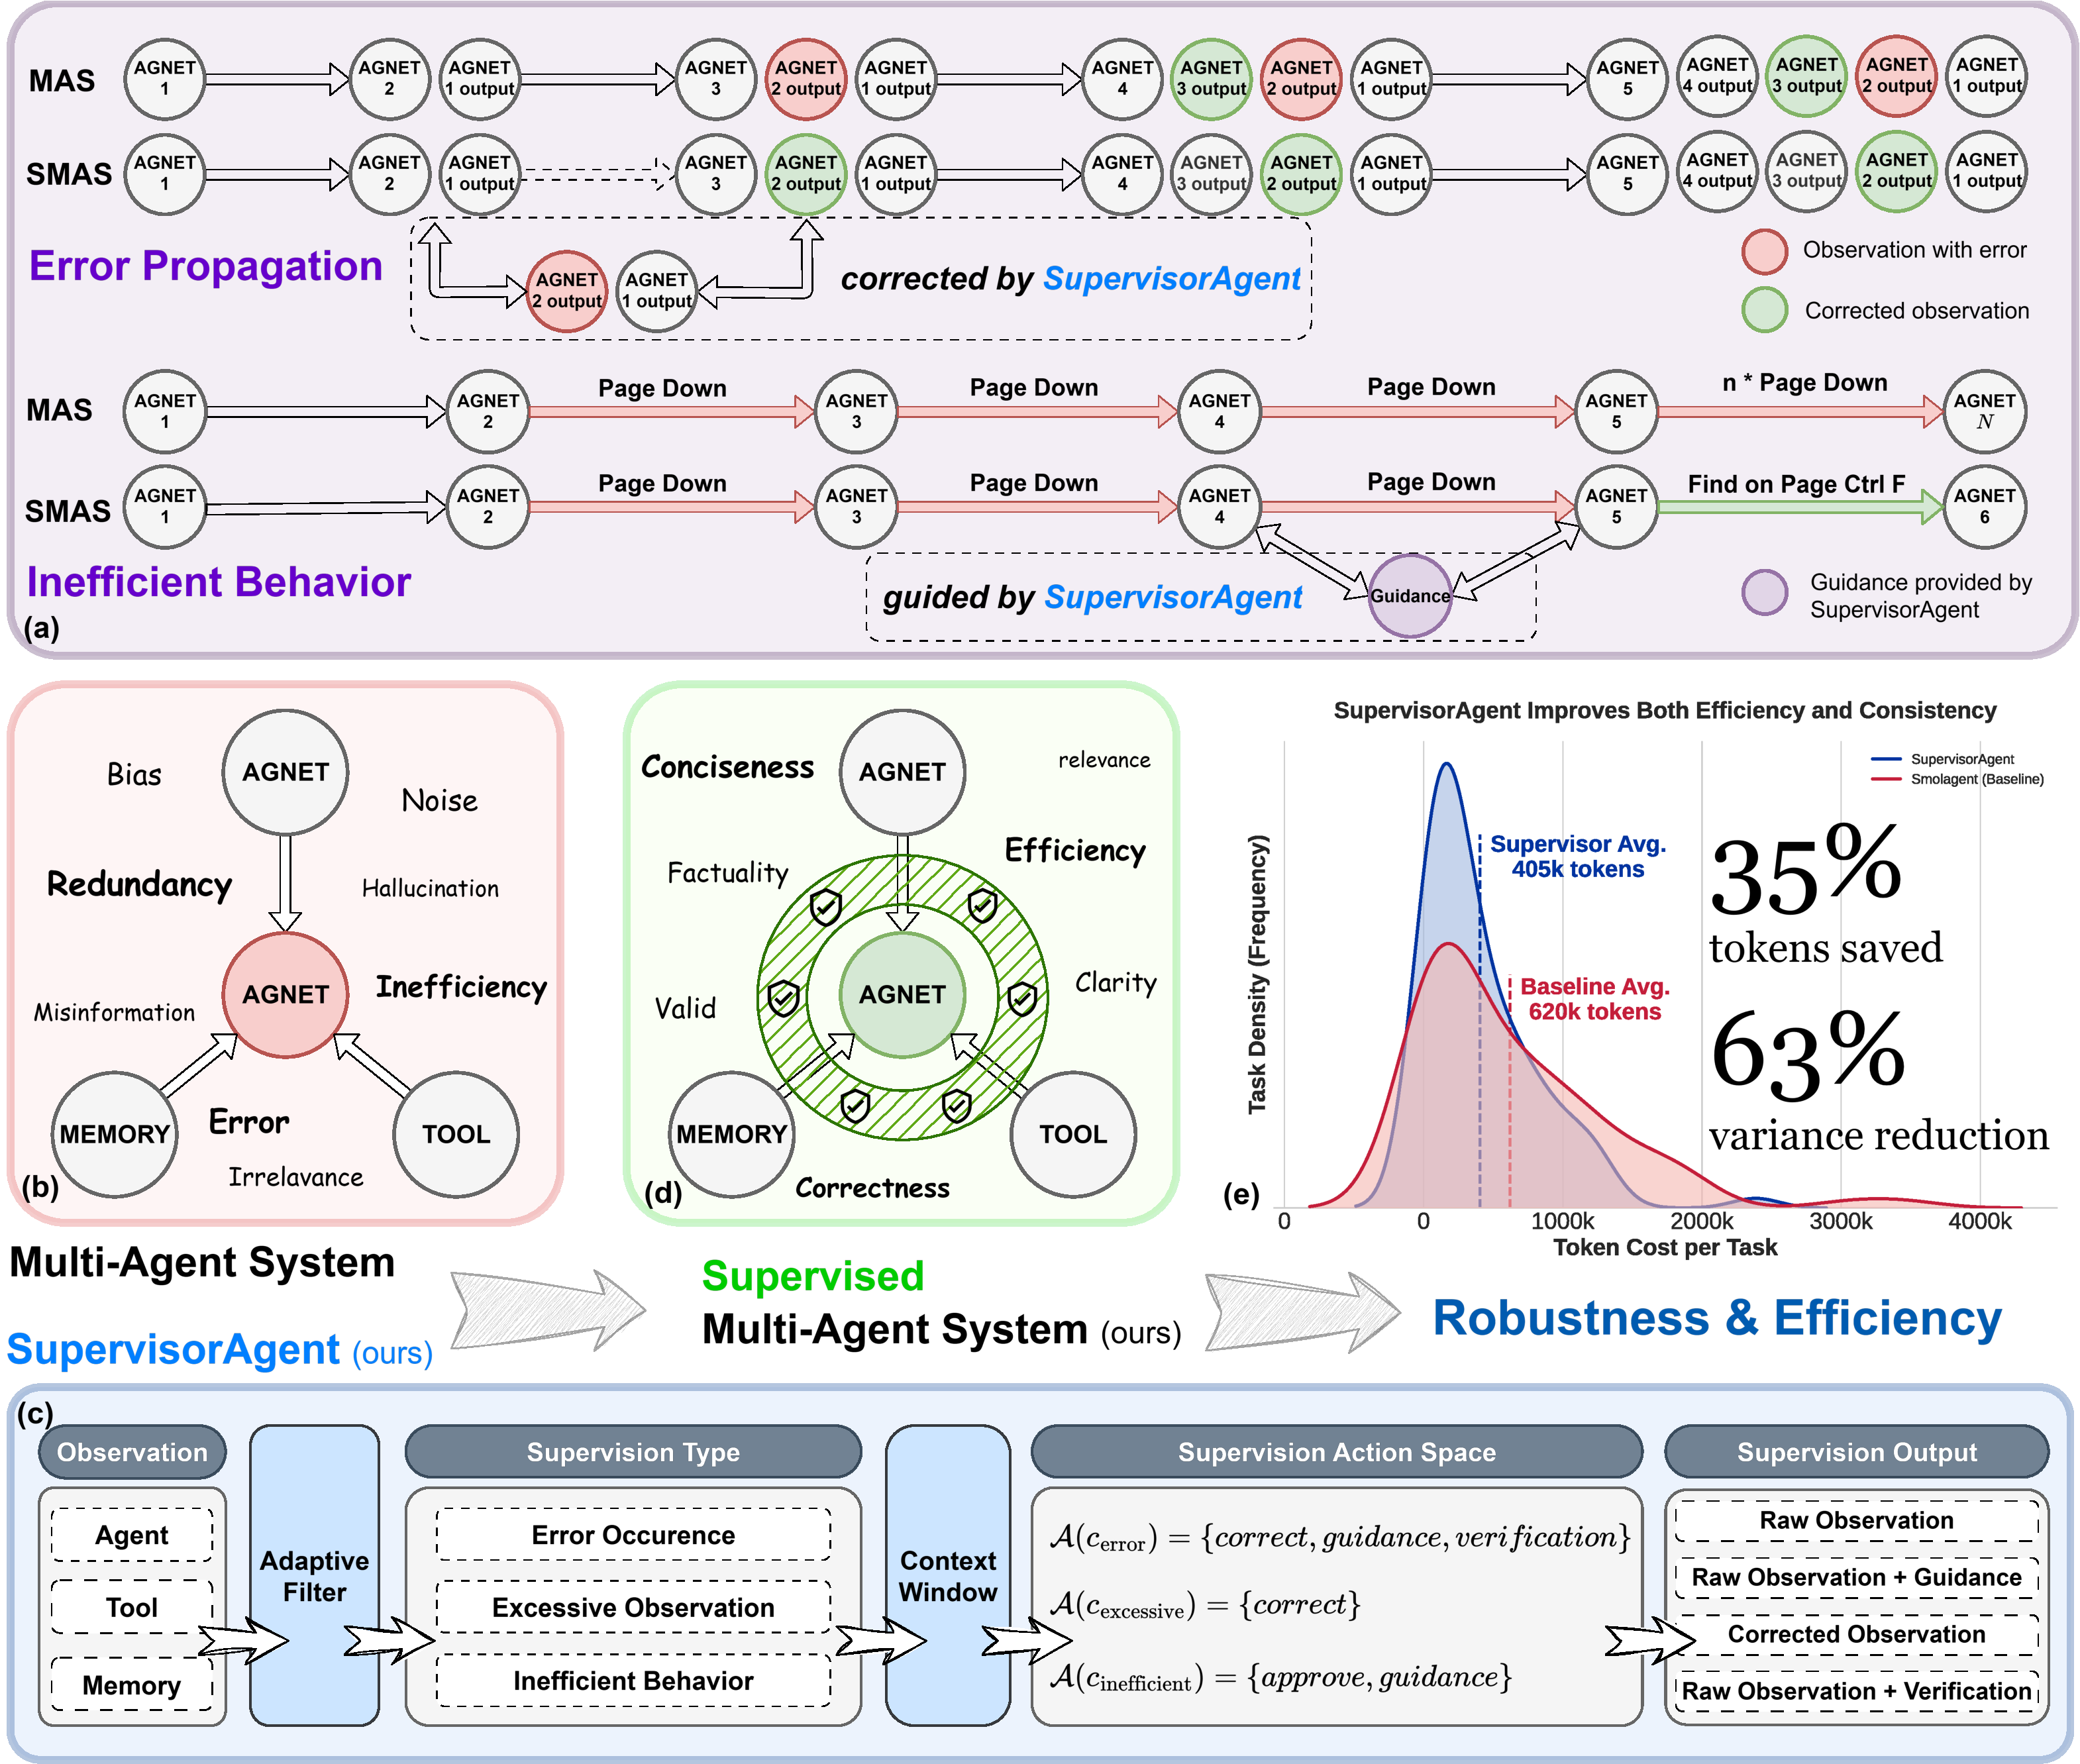
\includegraphics[width=0.9\linewidth]{resources/figures/introduction.pdf}
    \caption{\small
        \textbf{The \method Framework: Concept and Impact.}
        \textbf{(a)}~Illustrative examples of common failure modes in MAS, including \textbf{error propagation} and \textbf{inefficient loops}, and the corresponding intervention by our \method.
        \textbf{(b)}~An overview of a conventional MAS, highlighting the high-risk interaction loci (agent-agent, agent-tool, agent-memory) where such failures occur.
        \textbf{(c)}~The core workflow of our \method, which monitors these interactions to provide real-time intervention.
        \textbf{(d)}~The resulting Supervised MAS (SMAS), which integrates the \method to enhance robustness and efficiency.
        \textbf{(e)}~Performance on GAIA (Level 2), where SMAS (blue) reduces token cost by 35\% and variance by 63\% versus the baseline (red).
    }
    \vspace{-2em}
    \label{fig:introduction}
\end{figure}


\textbf{In summary, our main contributions are:}
\begin{enumerate}[nosep, leftmargin=12pt]
    \item We propose and implement \textbf{\method}, a novel, lightweight, and non-intrusive meta-agent framework for real-time MAS supervision.
          It improves agent robustness and efficiency through proactive error correction, inefficiency guidance, and adaptive observation purification, without altering the base agents' architecture.
    \item We conduct extensive experiments on the challenging \textbf{GAIA} benchmark and demonstrate a significant \textbf{Pareto improvement}.
          When applied to the Smolagent framework~\citep{smolagents}, \method reduces token consumption by an average of \textbf{29.68\%} while maintaining competitive task success rates.
    \item We validate the \textbf{general applicability} of our approach across five additional benchmarks spanning mathematical reasoning, code generation, and question answering.
          Our method consistently delivers substantial efficiency gains, highlighted by a \textbf{23.74\%} token reduction on HumanEval alongside an accuracy improvement.
          The framework's effectiveness is further confirmed across various foundation models, including the GPT-4.1, Gemini-2.5-pro, and Qwen3 series.
\end{enumerate}



\section{Related Work}

\paragraph{The increasing complexity of Multi-Agent Systems (MAS).}
Recent advancements in Large Language Models have spurred the development of increasingly sophisticated Multi-Agent Systems (MAS) capable of tackling complex, multi-step tasks~\citep{tran2025multiagentcollaborationmechanismssurvey,he2025llm}.
Frameworks like Tongyi DeepResearch~\citep{tongyidr}, AgentOrchestra~\citep{zhang2025agentorchestrahierarchicalmultiagentframework}, and Aime~\citep{shi2025aimefullyautonomousmultiagentframework} exemplify this trend, introducing complex features such as hierarchical structures~\citep{zhu2025oagentsempiricalstudybuilding,cheng2025hawkhierarchicalworkflowframework}, dynamic agent management~\citep{wu2025talkrightspecialistsrouting,zhang2025webpilot}, and end-to-end training~\citep{li2025chainofagentsendtoendagentfoundation,ye2025masgpttrainingllmsbuild}.
However, this escalating architectural complexity invariably introduces significant challenges in maintaining operational robustness and computational efficiency, which we address in this work.

\paragraph{Failure attribution and robustness.}
A significant body of work has emerged to address the challenge of MAS robustness, primarily focusing on post-hoc \textbf{\emph{failure attribution}}~\citep{zhang2025agentcausestaskfailures}.
Systems like Aegis~\citep{song2025aegistaxonomyoptimizationsovercoming} and SHIELDA~\citep{zhou2025shieldastructuredhandlingexceptions} propose taxonomies for failure analysis, while AgenTracer~\citep{zhang2025agentracerinducingfailurellm} and A2P~\citep{west2025abductactpredictscaffolding} introduce methods to better trace the root causes of task failures.
While valuable, these methods are fundamentally reactive, analyzing failures after they have occurred.
In contrast, our \method is designed for \textbf{\emph{proactive, real-time intervention}}, aiming to detect and mitigate high-risk steps \emph{before} they lead to systemic failure.


\paragraph{Efficient Multi-Agent Systems.}
Another stream of research targets the \textbf{efficiency} of MAS, a critical factor largely driven by token consumption. Most approaches focus on \emph{design-time optimization}. Some prune the system's architecture by eliminating agents with AgentDropout~\citep{wang2025agentdropoutdynamicagentelimination} or communication links with SafeSieve~\citep{zhang2025safesieveheuristicsexperienceprogressive}. Others generatively construct efficient prompts~\citep{han2025mapgdmultiagentpromptgradient} or agent topologies from the outset, as seen in MetaAgent~\citep{zhang2025metaagentautomaticallyconstructingmultiagent}, MaAS~\citep{zhang2025agentic-supernet}, and HiVA~\citep{tang2025hivaselforganizedhierarchicalvariable}. A second direction, \emph{context compression}, aims to reduce token count by summarizing or distilling observations~\citep{chen2025smurfs,mou2025ecolangefficienteffectiveagent}. Our work is orthogonal to these methods. Instead of focusing on static design or message content, we introduce \textbf{runtime process control}. \method addresses dynamic inefficiencies \emph{during} execution, a complementary approach that can enhance existing systems.



\section{Preliminary}
\label{sec:preliminary}
In this section, we first establish a formalism for our proposed \underline{S}upervised \underline{M}ulti-\underline{A}gent \underline{S}ystem (SMAS).
We then detail the core components of our framework: the \method's action space and the contextual information it leverages for decision-making.

\subsection{A Formalism for Supervised Multi-Agent Systems}
\label{sec:smas_formalism}
Our work is predicated on the idea that the complex, often chaotic, interactions within a Multi-Agent System (MAS; see Figure \ref{fig:introduction}b) can be actively managed to improve both robustness and efficiency.
To formalize this, we introduce the concept of a {Supervised Multi-Agent System} (SMAS; see Figure \ref{fig:introduction}d).


\begin{definition}[Supervised Multi-Agent System (SMAS)]
    A SMAS is a Multi-Agent System augmented with a meta-level control agent, henceforth referred to as the \textbf{Supervisor}. The Supervisor's objective is to monitor agent interactions in real-time, proactively detecting and mitigating operational risks without altering the core logic of the agents it oversees. In this work, we implement this conceptual Supervisor as a concrete agent named \textbf{\method}.
\end{definition}

The fundamental unit of supervision is the \textbf{interaction}, which occurs when an agent engages with other system components. We categorize interactions into three primary types:
\begin{enumerate}[nosep, leftmargin=12pt]
    \item \textbf{Agent-Agent Interactions:} Communication or delegation between agents.
          In architectures like ReAct~\citep{yao2023reactsynergizingreasoningacting}, where an agent's output becomes another's input, this channel is highly susceptible to the propagation of hallucinated or erroneous information~\citep{shen2025understandinginformationpropagationeffects};
    \item \textbf{Agent-Tool Interactions:}
          The invocation of external tools or APIs.
          This interaction is a primary source of external information, but it is also fraught with risks, including factually incorrect, irrelevant, or outdated data that can corrupt the agent's context~\citep{qian2025smartselfawareagenttool};
    \item \textbf{Agent-Memory Interactions:}
          The retrieval of information from short- or long-term memory stores.
          While crucial for self-evolving systems, memory introduces the hazard of acting upon stale or flawed information from past experiences~\citep{xiong2025memorymanagementimpactsllm}.
\end{enumerate}


\subsection{The \method's Context Window}


To make informed decisions, the \method is provided with a rich, real-time snapshot of the MAS's state, which we formalize as the \emph{context window}.

\begin{definition}[Context Window]
    The standard context window, $\mathcal{W}$, is a tuple of five key elements:
    \[
        \mathcal{W} = (N, Q_g, Q_l, T_l, S) \,,
    \]
    where $N$ is the name of the agent under review, $Q_g$ and $Q_l$ are the global and local tasks, $T_l$ is the \textbf{local trace} of agent $N$'s recent actions and observation summaries, and $S$ is a summary of the agent's latest interaction step.
    For diagnosing system-wide inefficiencies, we augment this to an extended context window $\mathcal{W}_{\text{ext}} = \mathcal{W} \cup \{T_g\}$, where $T_g$ is the \textbf{global trace} of all agent interactions.
\end{definition}






\subsection{The \method's Action Space}
The role of the \method is to diagnose high-risk interactions and execute a targeted intervention (Figure~\ref{fig:methodology}c). We define three primary intervention contexts, $c \in \mathcal{C} = \{c_{\text{error}}, c_{\text{inefficient}}, c_{\text{excessive}} \}$, which activate one of three core supervision strategies:

\begin{itemize}[nosep, leftmargin=12pt,labelindent=0pt]
    \item \textbf{Proactive Error Correction:} Triggered by $c_{\text{error}}$, this strategy aims to diagnose the root cause of an explicit error and provide a direct fix or a verification task to resolve it.
    \item \textbf{Guidance for Inefficiency:} Triggered by $c_{\text{inefficient}}$, this strategy provides pragmatic, course-correcting hints for sub-optimal behaviors, while also critically permitting productive, albeit repetitive, processes to continue via an \textit{approve} action.
    \item \textbf{Adaptive Observation Purification:} Triggered by $c_{\text{excessive}}$, this strategy refines excessively long or noisy observations to improve the signal-to-noise ratio for the agent.
\end{itemize}

These strategies are implemented by selecting an action $a$ from the global action space $\mathcal{A}$. The specific subset of permissible actions, $\mathcal{A}(c)$, is formally defined by the intervention context as follows:
\begin{align*}
    \mathcal{A}(c) =
    \begin{cases}
        \{ \textit{correct\_observation}, \textit{provide\_guidance}, \textit{run\_verification} \} & \text{if } c = c_{\text{error}}       \\
        \{ \textit{approve}, \textit{provide\_guidance} \}                                          & \text{if } c = c_{\text{inefficient}} \\
        \{ \textit{correct\_observation} \}                                                         & \text{if } c = c_{\text{excessive}}
    \end{cases}
\end{align*}
The implementation of each action is detailed in Section~\ref{sec:methodology_action}.



\section{Methodology}
\label{sec:methodology}

\begin{figure}[!t] %
    \centering
    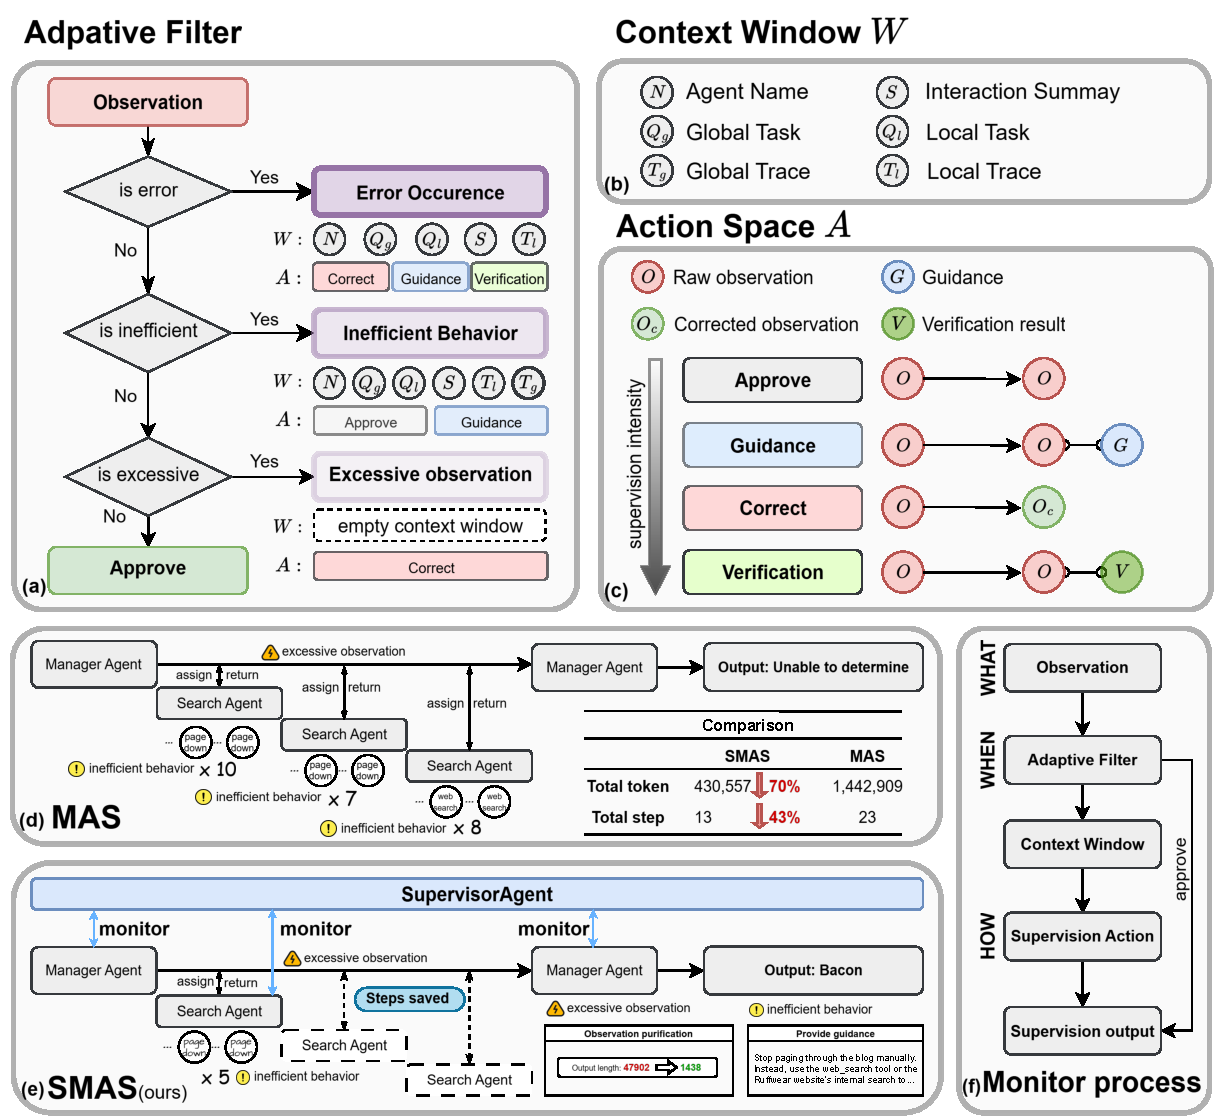
\includegraphics[width=0.9\linewidth]{resources/figures/methodology.pdf}
    \caption{
        \textbf{The architecture and workflow of \method.}
        \textbf{(a)} The LLM-free adaptive filter for identifying high-risk interactions.
        \textbf{(b)} The context window, aggregating goals and traces for situational awareness.
        \textbf{(c)} The spectrum of intervention actions, from simple approval to intensive verification.
        \textbf{(d, e)} Case study on a GAIA task, comparing the baseline MAS (d) with our SMAS (e), which cuts steps by 43\% and token cost by over 70\%.
        \textbf{(f)} The supervise workflow for an interaction, from filtering to a final supervision action.
    }
    \vspace{-1em}
    \label{fig:methodology}
\end{figure}


Building upon the formalism of a Supervised Multi-Agent System (SMAS) introduced in Section~\ref{sec:preliminary}, we now detail the architecture and operational workflow of our \method (illustrated in Figure~\ref{fig:methodology}). Our methodology is structured around three fundamental questions: \textbf{What} to supervise, \textbf{When} to supervise, and \textbf{How} to supervise. We defer the specific implementation details, including all hyperparameters and prompts, to Appendix~\ref{implementation_details} and~\ref{appendix:prompt}.

\subsection{What to Supervise: High-Risk Interaction Points}
The primary targets for our supervision are the three high-risk interaction points defined in our preliminary formalism (Section~\ref{sec:smas_formalism}, see also Figure~\ref{fig:methodology}a): Agent-Agent, Agent-Tool, and Agent-Memory interactions. These points are the primary channels through which errors and inefficiencies are introduced and propagated throughout the system. Our goal is to monitor these specific channels to maintain the operational integrity of the MAS.

\subsection{When to Supervise: The Adaptive Filter}
While a naive approach might monitor every interaction, the associated computational cost is prohibitive and would undermine our goal of improving efficiency.
Therefore, the cornerstone of our framework is a lightweight, LLM-free \textbf{adaptive filter} (see in Figure\ref{fig:methodology}a) designed to trigger supervision only at critical junctures (see case studies in Figures~\ref{fig:methodology}d and~\ref{fig:methodology}e).
This approach ensures that the \method's resources are deployed judiciously, maximizing impact while minimizing overhead.
The filter is designed to be fast and heuristic-based, monitoring the MAS for three pre-defined, high-risk scenarios:
\looseness=-1
\begin{itemize}[nosep, leftmargin=12pt]
    \item \textbf{Error occurrence:}
          The manifestation of an explicit error (e.g., in tool use or code execution) is a critical trigger.
          Unlike current MAS that often pass the full error log into a cluttered context for a subsequent agent to debug, our filter immediately flags these events for a focused, real-time intervention.
          \looseness=-1

    \item \textbf{Inefficient behavior:}
          An agent may enter a loop of sub-optimal or repetitive actions that, while not explicit errors, lead to high token consumption and latency.
          Our filter is designed to detect such patterns, such as an agent repeatedly using the \texttt{page\_down} action instead of a more direct search strategy.
          \looseness=-1

    \item \textbf{Excessive observation length:}
          Interactions with tools can return excessively long and noisy observations (e.g., raw HTML) that inflate costs and distract the agent.
          Our filter identifies such cases for immediate information purification.
          \looseness=-1
\end{itemize}



\subsection{How to Supervise: Memory-Augmented, Multi-Level Intervention}
\label{sec:methodology_action}
Once a high-risk interaction is flagged, \method leverages a rich context window and a spectrum of intervention strategies to deliver a nuanced, effective response.

\paragraph{Memory-augmented context window.} To make an effective decision, a supervisor must possess a more comprehensive understanding of the system's state than any single agent.
This is why \method is conceptualized with its own memory module, not a simple monitor.
As illustrated in Figure~\ref{fig:methodology}b, this is achieved through a dynamic \textbf{context window} $\mathcal{W}$, which aggregates the global task $Q_g$, the agent's local task $Q_l$, interaction summary $S$, and its recent local action trace $T_l$.
Crucially, for diagnosing complex inefficiencies, \method also accesses the \textbf{global trace} $T_g$, granting it a holistic perspective that transcends the limited view of any individual agent.
This elevated viewpoint is what enables it to provide genuinely strategic guidance.

\paragraph{A spectrum of intervention actions.}
With this rich context, \method selects an action from a multi-level action space $\mathcal{A}$, adapting intervention intensity tailored to issue severity (Figure~\ref{fig:methodology}c).
These actions range from a minimal nudge to a comprehensive correction:
\begin{itemize}[nosep, leftmargin=15pt]
    \item \emph{\textbf{approve}}: A minimal intervention that permits a productive, albeit repetitive, agent behavior to continue. Primarily used in the \emph{inefficient} context, its purpose is to avoid disrupting a process that is pragmatically the best path forward from its current state.
    \item \emph{\textbf{provide\_guidance}}: A semi-intrusive action that steers an agent away from a sub-optimal strategy or logical flaw. This action appends a concise, directive hint to the existing observation, correcting the agent's reasoning path without altering the core context data.
    \item \emph{\textbf{correct\_observation}}: A direct and forceful intervention that refines the agent's sensory input. It is the sole action for \emph{excessive observations}, where it purifies the content, and is also used in \emph{error} contexts to fix factually incorrect data.
          This action replaces the original raw observation entirely with a cleaned and corrected version.
    \item \emph{\textbf{run\_verification}}: The deepest intervention, used in complex \emph{error} contexts when internal information is insufficient.
          It invokes a verification sub-agent for external fact-checking or advanced debugging, returning a definitive, verified result.
\end{itemize}


\section{Experiments}
\label{sec:experiments}

\subsection{Experimental Setup}
We empirically validate the effectiveness of \method through a series of extensive experiments.
We begin by outlining our evaluation metrics, datasets, and baselines.
For a more detailed description of the experimental settings, please refer to Appendix \ref{experiment_details}.

\paragraph{Datasets.}
We evaluate our method on a diverse suite of six benchmarks spanning three domains.
Our primary benchmark is the challenging GAIA validation set~\citep{mialon2023gaiabenchmarkgeneralai}, which provides a comprehensive test of an MAS's general problem-solving capabilities.
To demonstrate broader applicability, we use five additional benchmarks: for mathematical reasoning, we use AIME 2024~\citep{HuggingFaceH4_AIME_2024} and a random subset of 600 samples from GSM8k-Hard~\citep{gao2022pal}; for code generation, we use the full HumanEval~\citep{chen2021evaluatinglargelanguagemodels} and MBPP~\citep{austin2021programsynthesislargelanguage} datasets; and for question answering, we use a subset of 800 samples from the DROP~\citep{dua-etal-2019-drop} dataset, following the sampling strategy of prior work~\citep{zhang2025aflowautomatingagenticworkflow}.

\paragraph{Baselines.}
On several benchmarks, we compare \method against a comprehensive set of agentic systems equipped with web-browsing and code execution capabilities.
These baselines fall into two categories: (1) single agent execution methods: including vanilla LLM, Self Consistency CoT (3 answers)~\citep{wang2023selfconsistencyimproveschainthought}, and CodeAgent~\citep{smolagents}; and (2) multi-agent systems, including Smolagent~\citep{smolagents}, OAgents~\citep{zhu2025oagentsempiricalstudybuilding}, MetaAgent~\citep{zhang2025metaagentautomaticallyconstructingmultiagent}, OWL (role playing)~\citep{hu2025owl}, and AWorld~\citep{xie2025profileawaremaneuveringdynamicmultiagent,yu2025aworldorchestratingtrainingrecipe}. 
Detailed descriptions of these baselines are provided in Appendix~\ref{appendix:baselines}.

\paragraph{Implementation details.}
To assess model-agnosticism, we test \method with multiple foundation models.
For the demanding GAIA benchmark, we primarily use GPT-4.1 as the base model for all agents, and evaluate \method when powered by GPT-4.1~\citep{openai_gpt4.1_2025}, Gemini-2.5-pro-0605~\citep{comanici2025gemini25pushingfrontier}, and Qwen3-235B-2507~\citep{qwen3technicalreport}.
For all other benchmarks, we employ the efficient and powerful Qwen3-32B~\citep{qwen3technicalreport} for both the base agents and the \method to assess performance in a more resource-constrained setting.


\paragraph{Testbed selection.}
We selected Smolagent as our primary experimental testbed, which provides a flexible framework upon which we build our agentic systems (SMAS). Critically, Smolagent's capabilities stem primarily from its internal agentic interactions rather than powerful external tools(e.g. web APIs or solvers). This provides an ideal, controlled environment to isolate and evaluate the direct impact of our \method on an agent's core reasoning and communication processes.



\paragraph{Metrics.}
For GAIA and the code generation benchmarks, we report the standard pass@k metric.
For our main baseline, Smolagent, we report pass@1, 2, and 3.
For math reasoning, we report the final solve rate (\%).
For question answering, we report the F1 score for DROP.
In all experiments, we meticulously track and report the total token consumption as a primary measure of efficiency.



\begin{table}[!t]
    \caption{
        \textbf{Overall performance on the GAIA validation set. }
        Our SMAS consistently reduces the average token cost comparing to Smolagent baseline while achieving competitive pass@k success rates.
    }
    \label{tab:multiagent-results}
    \centering
    \resizebox{\textwidth}{!}{
        \begin{tabular}{@{}lcccccccc@{}}
            \toprule
            \multicolumn{1}{c}{\bf Method}                & \multicolumn{1}{c}{\bf Avg. Acc.}              & \multicolumn{1}{c}{\bf Avg. Tokens (K)}        & \multicolumn{1}{c}{\bf L1 Acc.} & \multicolumn{1}{c}{\bf L1 Tokens (K)} & \multicolumn{1}{c}{\bf L2 Acc.} & \multicolumn{1}{c}{\bf L2 Tokens (K)} & \multicolumn{1}{c}{\bf L3 Acc.} & \multicolumn{1}{c}{\bf L3 Tokens (K)} \\
            \midrule
            CodeAgent                                     & 40.00                                          & 120.40                                         & 56.60                           & 92.84                                 & 34.88                           & 131.90                                & 23.08                           & 138.54                                \\
            OWL                                           & 45.40                                          & 111.07                                         & 56.56                           & 67.72                                 & 43.02                           & 110.36                                & 29.16                           & 209.34                                \\
            OAgents                                       & 49.09                                          & 340.50                                         & 66.04                           & 260.27                                & 47.67                           & 358.63                                & 19.23                           & 444.11                                \\
            Smolagent                                     & 50.91                                          & 527.76                                         & 62.26                           & 298.51                                & 53.49                           & 619.59                                & 19.23                           & 691.33                                \\
            AWorld                                        & 60.00                                          & 128.27                                         & 67.92                           & 69.61                                 & 62.79                           & 164.08                                & 34.62                           & 133.65                                \\
            \midrule
            \multicolumn{9}{c}{\bf pass@1}                                                                                                                                                                                                                                                                                                                                                \\
            \midrule
            Smolagent                                     & 50.91                                          & 527.76                                         & 62.26                           & 298.51                                & 53.49                           & 619.59                                & 19.23                           & 691.33                                \\
            \, + \textbf{SMAS (ours)}                     & 50.91                                          & 371.12 {\scriptsize \textcolor{red}{↓29.68\%}} &
            62.26                                         & 258.28 {\scriptsize \textcolor{red}{↓13.48\%}} &
            51.16                                         & 404.96 {\scriptsize \textcolor{red}{↓34.64\%}} &
            26.92 {\scriptsize \textcolor{blue}{↑7.69\%}} & 489.22 {\scriptsize \textcolor{red}{↓29.23\%}}                                                                                                                                                                                                                                                                                \\
            \midrule
            \multicolumn{9}{c}{\bf pass@2}                                                                                                                                                                                                                                                                                                                                                \\
            \midrule
            Smolagent                                     & 58.18                                          & 467.19                                         & 69.81                           & 275.85                                & 59.30                           & 548.02                                & 30.77                           & 589.92                                \\
            \, + \textbf{SMAS (ours)}                     & 58.79 {\scriptsize \textcolor{blue}{↑0.61\%}}  & 389.54 {\scriptsize \textcolor{red}{↓16.62\%}} &
            73.58 {\scriptsize \textcolor{blue}{↑3.77\%}} & 270.07 {\scriptsize \textcolor{red}{↓2.10\%}}  &
            56.98                                         & 420.97 {\scriptsize \textcolor{red}{↓23.18\%}} &
            34.62 {\scriptsize \textcolor{blue}{↑3.85\%}} & 529.20 {\scriptsize \textcolor{red}{↓10.29\%}}                                                                                                                                                                                                                                                                                \\
            \midrule
            \multicolumn{9}{c}{\bf pass@3}                                                                                                                                                                                                                                                                                                                                                \\
            \midrule
            Smolagent                                     & 61.82                                          & 502.40                                         & 71.70                           & 282.14                                & 63.95                           & 605.05                                & 34.62                           & 611.87                                \\
            \, + \textbf{SMAS (ours)}                     & 63.03 {\scriptsize \textcolor{blue}{↑1.21\%}}  & 369.52 {\scriptsize \textcolor{red}{↓26.45\%}} &
            75.47 {\scriptsize \textcolor{blue}{↑3.77\%}} & 276.84 {\scriptsize \textcolor{red}{↓1.88\%}}  &
            62.79                                         & 409.05 {\scriptsize \textcolor{red}{↓32.39\%}} &
            38.46 {\scriptsize \textcolor{blue}{↑3.84\%}} & 427.72 {\scriptsize \textcolor{red}{↓30.10\%}}                                                                                                                                                                                                                                                                                \\
            \bottomrule
        \end{tabular}
    }
\end{table}


\subsection{Results and Analysis}
\paragraph{Significant efficiency gains with competitive accuracy.}
The main experimental results, presented in Table \ref{tab:multiagent-results}, confirm the substantial benefits of \method.
On the GAIA validation set, when integrated with the Smolagent framework, \method achieves an average token reduction of \textbf{29.68\%} at pass@1, while maintaining a statistically equivalent success rate.
Notably, the efficiency gains are even more pronounced on more difficult tasks, with token savings reaching \textbf{32.39\%} on Level 2 and \textbf{30.10\%} on Level 3 tasks at pass@3.

\emph{Across the other five benchmarks, \method generally achieves a Pareto improvement} (see Table \ref{tab:benchmark-generalization}).
In mathematical reasoning, it raises the AIME solve rate by \textbf{6.67\%} while cutting token costs by \textbf{18.92\%}.
In code generation, it maintains competitive accuracy on HumanEval and further reduces token use by \textbf{23.74\%}, likely due to its ability to streamline repetitive debugging cycles.
Occasionally, \method may overcompress long contexts during purification, causing minor accuracy or F1 drops on certain benchmarks.
These results underscore \method's ability to act as a universal efficiency enhancer across diverse problem domains.
\looseness=-1


\begin{table}[!t]
    \caption{
        \textbf{Generalization across diverse benchmarks.}
        \method consistently reduces token costs while maintaining or improving accuracy on tasks spanning mathematical reasoning, code generation, and question answering. All reported gains are relative to the Smolagent baseline.
    }
    \label{tab:benchmark-generalization}
    \centering
    \resizebox{\textwidth}{!}{%
        \begin{tabular}{@{}llccccc@{}}
            \toprule
            \textbf{Method}                            & \textbf{Metrics} & \textbf{GSM-hard}                            & \textbf{AIME}                                 & \textbf{HumanEval}                            & \textbf{MBPP}                                 & \textbf{DROP}                                \\ \midrule
            \multirow{2}{*}{Vanilla}                   & Acc / F1 (\%)    & 67.17                                        & 26.67                                         & 76.82                                         & 80.09                                         & 76.36                                        \\
                                                       & Avg. Tokens (K)  & 0.37                                         & 2.01                                          & 0.28                                          & 0.27                                          & 0.46                                         \\ \cmidrule(l){2-7}
            \multirow{2}{*}{CoT SC (3-shot)}           & Acc / F1 (\%)    & 69.01                                        & 30.00                                         & 77.78                                         & 81.26                                         & 77.72                                        \\
                                                       & Avg. Tokens (K)  & 2.62                                         & 14.26                                         & 1.42                                          & 1.29                                          & 2.73                                         \\ \cmidrule(l){2-7}
            \multirow{2}{*}{OWL}                       & Acc / F1 (\%)    & 72.48                                        & 33.33                                         & 90.74                                         & 79.08                                         & 79.85                                        \\
                                                       & Avg. Tokens (K)  & 15.67                                        & 56.11                                         & 31.87                                         & 54.80                                         & 11.47                                        \\ \cmidrule(l){2-7}
            \multirow{2}{*}{MetaAgent}                 & Acc / F1 (\%)    & 72.14                                        & 26.67                                         & 74.08                                         & 79.86                                         & 78.16                                        \\
                                                       & Avg. Tokens (K)  & 4.35                                         & 6.24                                          & 2.59                                          & 6.39                                          & 1.43                                         \\ \midrule
            \multirow{2}{*}{Smolagent}                 & Acc / F1 (\%)    & 74.33                                        & 30.00                                         & 92.07                                         & 85.68                                         & 81.08                                        \\
                                                       & Avg. Tokens (K)  & 11.59                                        & 59.14                                         & 40.91                                         & 111.07                                        & 12.01                                        \\ \cmidrule(l){2-7}
            \multirow{2}{*}{\, + \textbf{SMAS (ours)}} & Acc / F1 (\%)    & 75.50                                        & 36.67                                         & 92.68                                         & 84.43                                         & 79.80                                        \\
                                                       & Avg. Tokens (K)  & 10.55 {\scriptsize \textcolor{red}{↓8.92\%}} & 47.95 {\scriptsize \textcolor{red}{↓18.92\%}} & 31.19 {\scriptsize \textcolor{red}{↓23.74\%}} & 103.71 {\scriptsize \textcolor{red}{↓6.62\%}} & 11.34 {\scriptsize \textcolor{red}{↓5.60\%}} \\ \bottomrule
        \end{tabular}%
    }
\end{table}




\begin{figure}[!t] %
    \centering
    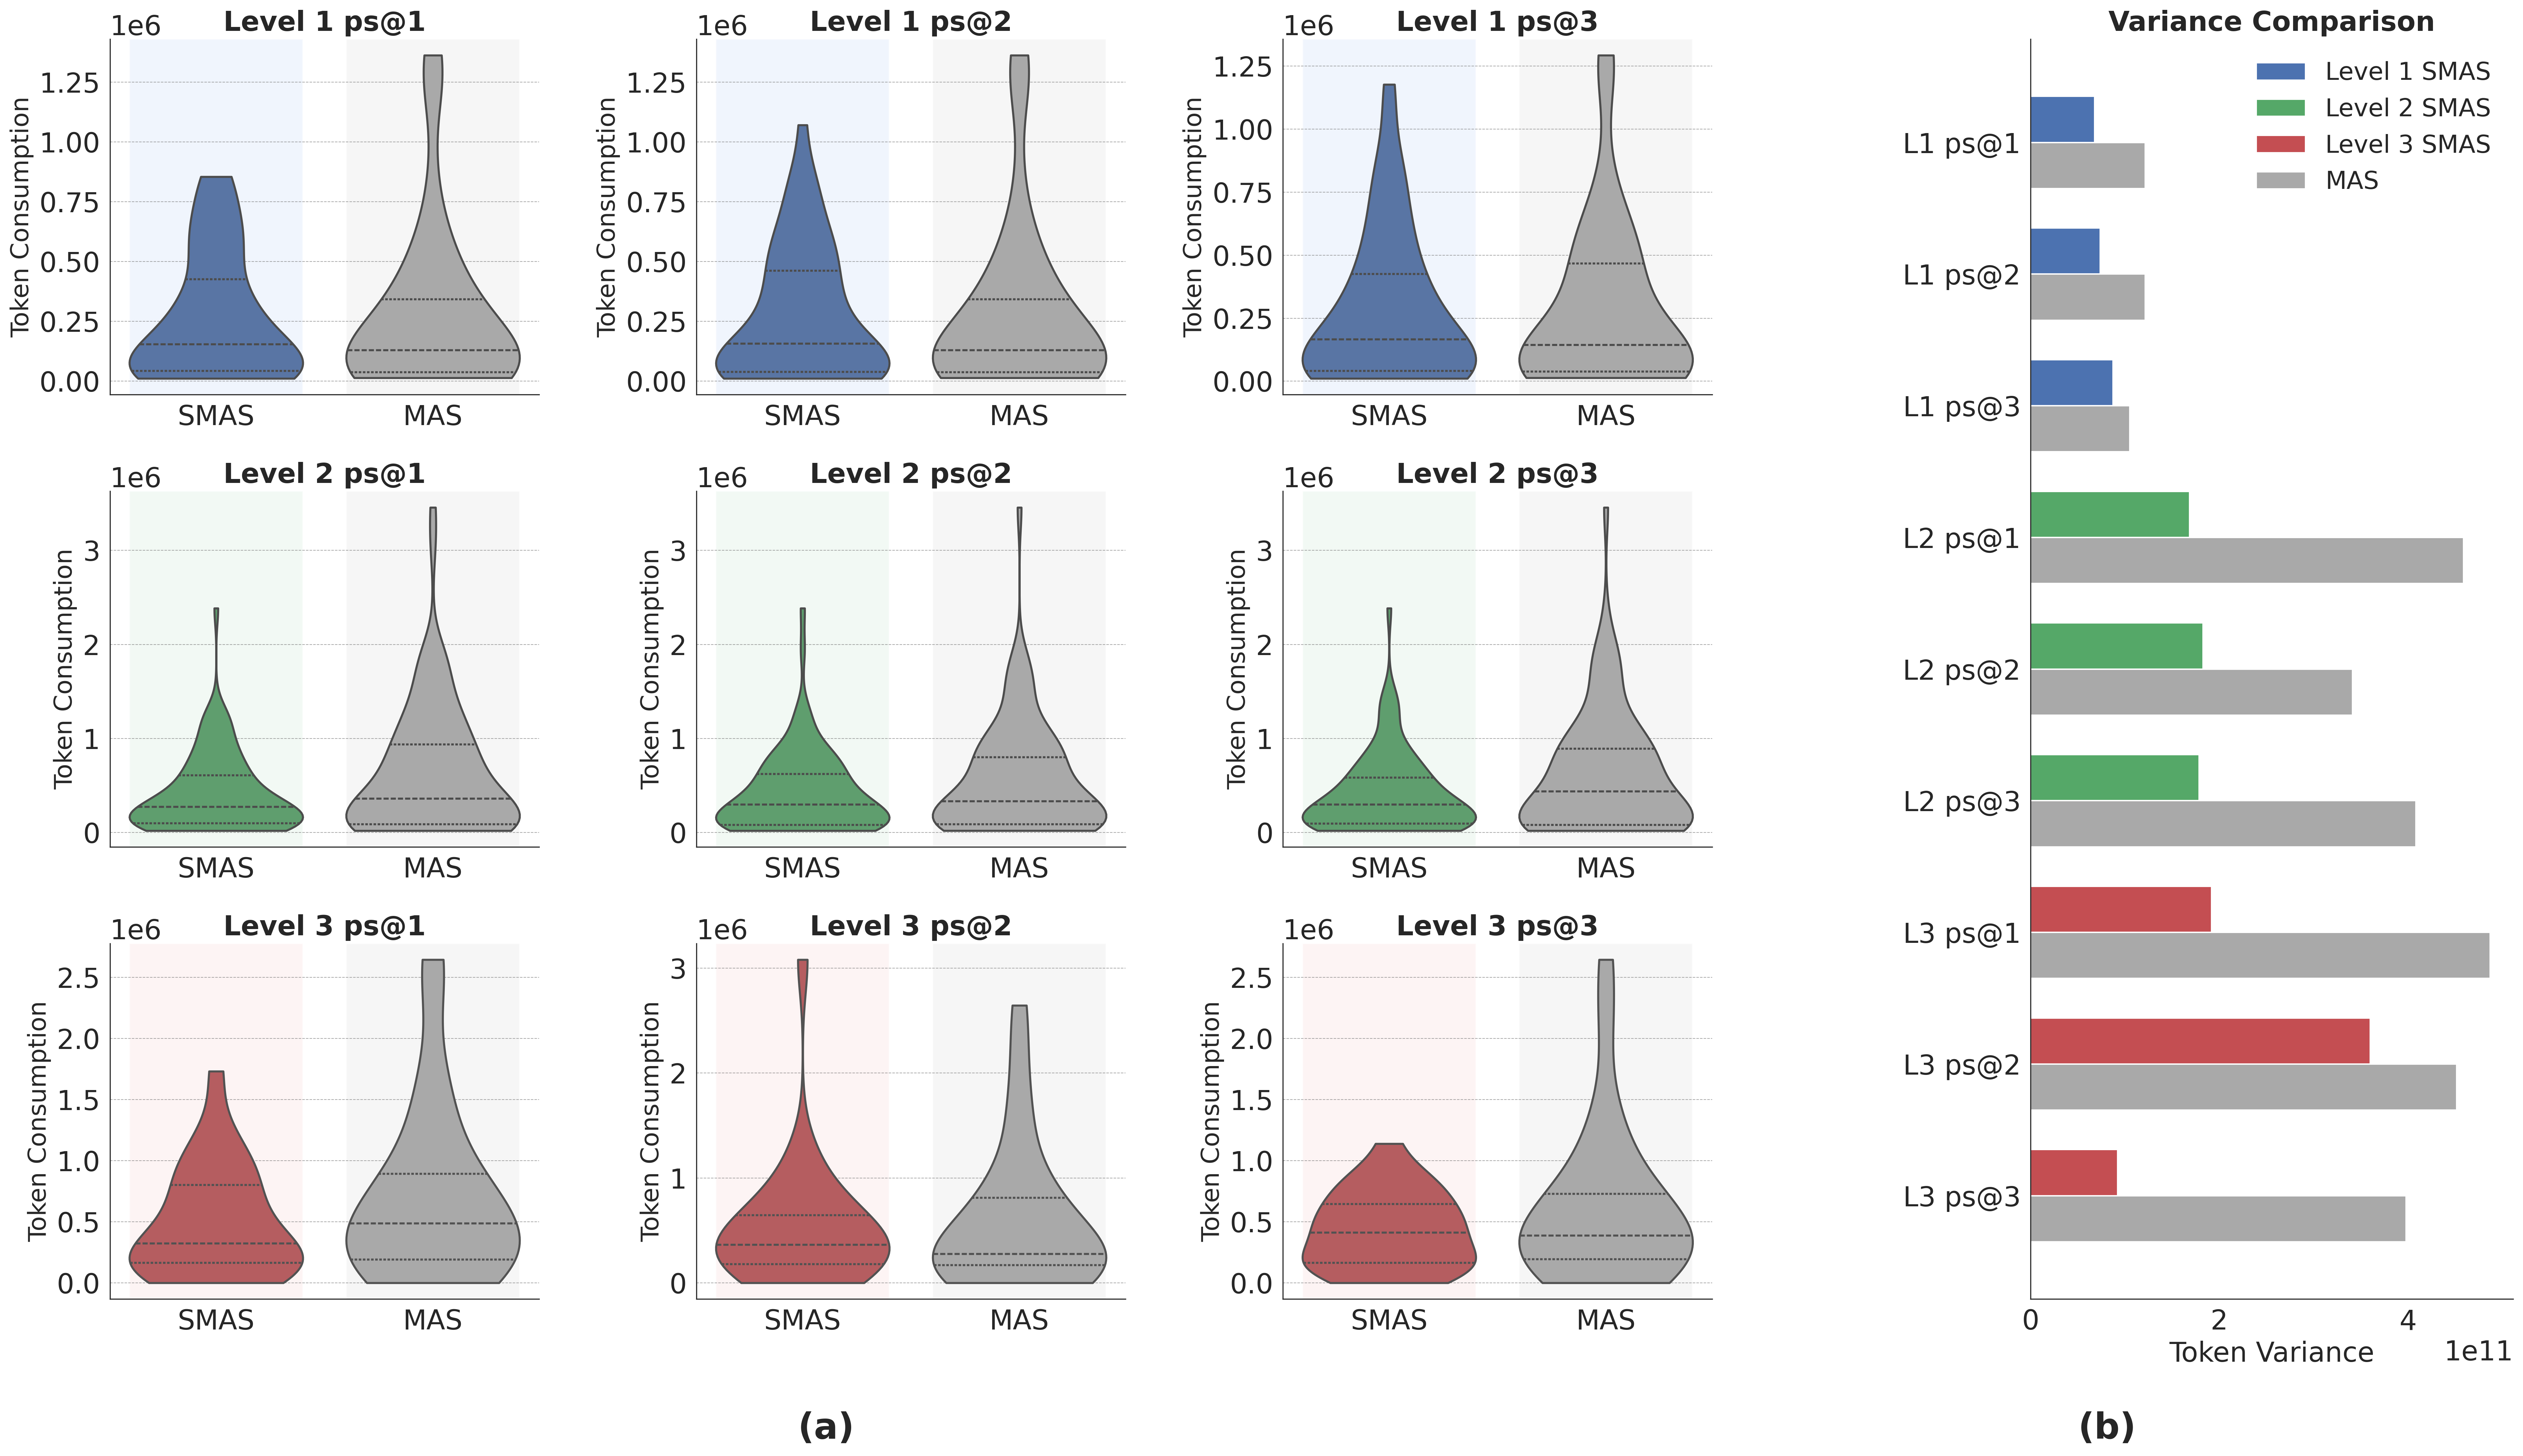
\includegraphics[width=0.9\linewidth]{resources/figures/violin_and_variance.png}
    \vspace{-0.5em}
    \caption{
        \textbf{\method enhances performance consistency on the GAIA benchmark.}
        \textbf{(a)} Violin plots of token cost distributions, revealing the more compact and predictable performance of our Supervised MAS (SMAS).
        \textbf{(b)} A direct comparison quantifying the substantial reduction in token cost variance achieved by our SMAS across all difficulty levels.
    }
    \label{fig:violin}
\end{figure}


\paragraph{Model-Agnostic generalization.}
To demonstrate that the benefits of \method are architectural rather than model-specific, we evaluated it with three different powerful LLMs as its inference engine on GAIA.
As shown in Figure \ref{fig:model-agnostic}, \emph{\method consistently yields significant token savings and maintains robust performance across all models, including GPT-4.1, Gemini-2.5-pro, and Qwen3-235B.}
This validates that our supervision framework is a model-agnostic component that can enhance a wide variety of LLM-powered agent systems.

\paragraph{Improving robustness and performance consistency.}
Beyond average performance, we define robustness as the consistency of an agent's performance.
As illustrated by the violin plots in Figure \ref{fig:violin}, \emph{\method significantly reduces the variance in token consumption per task.}
The distributions for the SMAS are visibly shorter and wider, indicating a more concentrated and predictable performance profile.
The bar chart on the right further quantifies this, showing a marked decrease in token cost variance, especially for the more complex Level 2 and 3 tasks.
This demonstrates that \emph{our method not only makes the MAS more efficient on average but also more reliable and less prone to extreme resource consumption outliers.}


\paragraph{Ablation study.} We conducted an ablation study on the full GAIA validation set to isolate the impact of \method's three core strategies (Table~\ref{tab:ablation_full}, Figure~\ref{fig:ablation}). A comparison of the full framework with \textbf{w/o Correction} (Proactive Error Correction), \textbf{w/o Guidance} (Guidance for Inefficiency), and \textbf{w/o Purification} (Adaptive Observation Purification) reveals distinct roles. \textbf{Purification} is the primary driver of efficiency; disabling it drastically reduces token savings (from 29.68\% to 15.96\%). Conversely, removing \textbf{Correction} or \textbf{Guidance} results in the most significant accuracy drops, confirming their necessity for robustness. This underscores a synergistic design: while Purification minimizes cost, Correction and Guidance ensure task success, justifying their marginal overhead. These benefits are particularly pronounced on high-cost tasks (see Appendix \ref{ablation_study_subset}).

\begin{table}[!t]
    \caption{
        \textbf{Ablation study of \method's components} on the full GAIA validation set.
    }
    \label{tab:ablation_full}
    \centering
    \resizebox{\textwidth}{!}{
        \begin{tabular}{>{\raggedright\arraybackslash}m{4cm} c c c c c}
            \toprule
            \bf Method                   & \bf Avg. Acc. & \bf Avg. Token                                   & \bf Level 1 Avg. Token                           & \bf Level 2 Avg. Token                           & \bf Level 3 Avg. Token                           \\
            \midrule
            Smolagent                    & 50.91         & 527,759                                          & 298,506                                          & 619,591                                          & 691,331                                          \\
            \, + SMAS (w/o Correction)   & 47.88         & 354,226 {\scriptsize \textcolor{blue}{↓32.88\%}} & 221,515 {\scriptsize \textcolor{blue}{↓25.79\%}} & 363,871 {\scriptsize \textcolor{blue}{↓41.27\%}} & 592,852 {\scriptsize \textcolor{blue}{↓14.24\%}} \\
            \, + SMAS (w/o Guidance)     & 48.48         & 363,644 {\scriptsize \textcolor{blue}{↓31.10\%}} & 253,591 {\scriptsize \textcolor{blue}{↓15.05\%}} & 419,913 {\scriptsize \textcolor{blue}{↓32.23\%}} & 401,861 {\scriptsize \textcolor{blue}{↓41.87\%}} \\
            \, + SMAS (w/o Purification) & 49.70         & 443,520 {\scriptsize \textcolor{blue}{↓15.96\%}} & 270,058 {\scriptsize \textcolor{blue}{↓9.53\%}}  & 502,937 {\scriptsize \textcolor{blue}{↓18.83\%}} & 600,582 {\scriptsize \textcolor{blue}{↓13.13\%}} \\
            \, + SMAS                    & 50.91         & 371,119 {\scriptsize \textcolor{blue}{↓29.68\%}} & 258,279 {\scriptsize \textcolor{blue}{↓13.48\%}} & 404,955 {\scriptsize \textcolor{blue}{↓34.64\%}} & 489,222 {\scriptsize \textcolor{blue}{↓29.23\%}} \\
            \bottomrule
        \end{tabular}
    }
\end{table}



\begin{figure}[!t]
    \centering
    \begin{subfigure}[t]{0.45\textwidth}
        \centering
        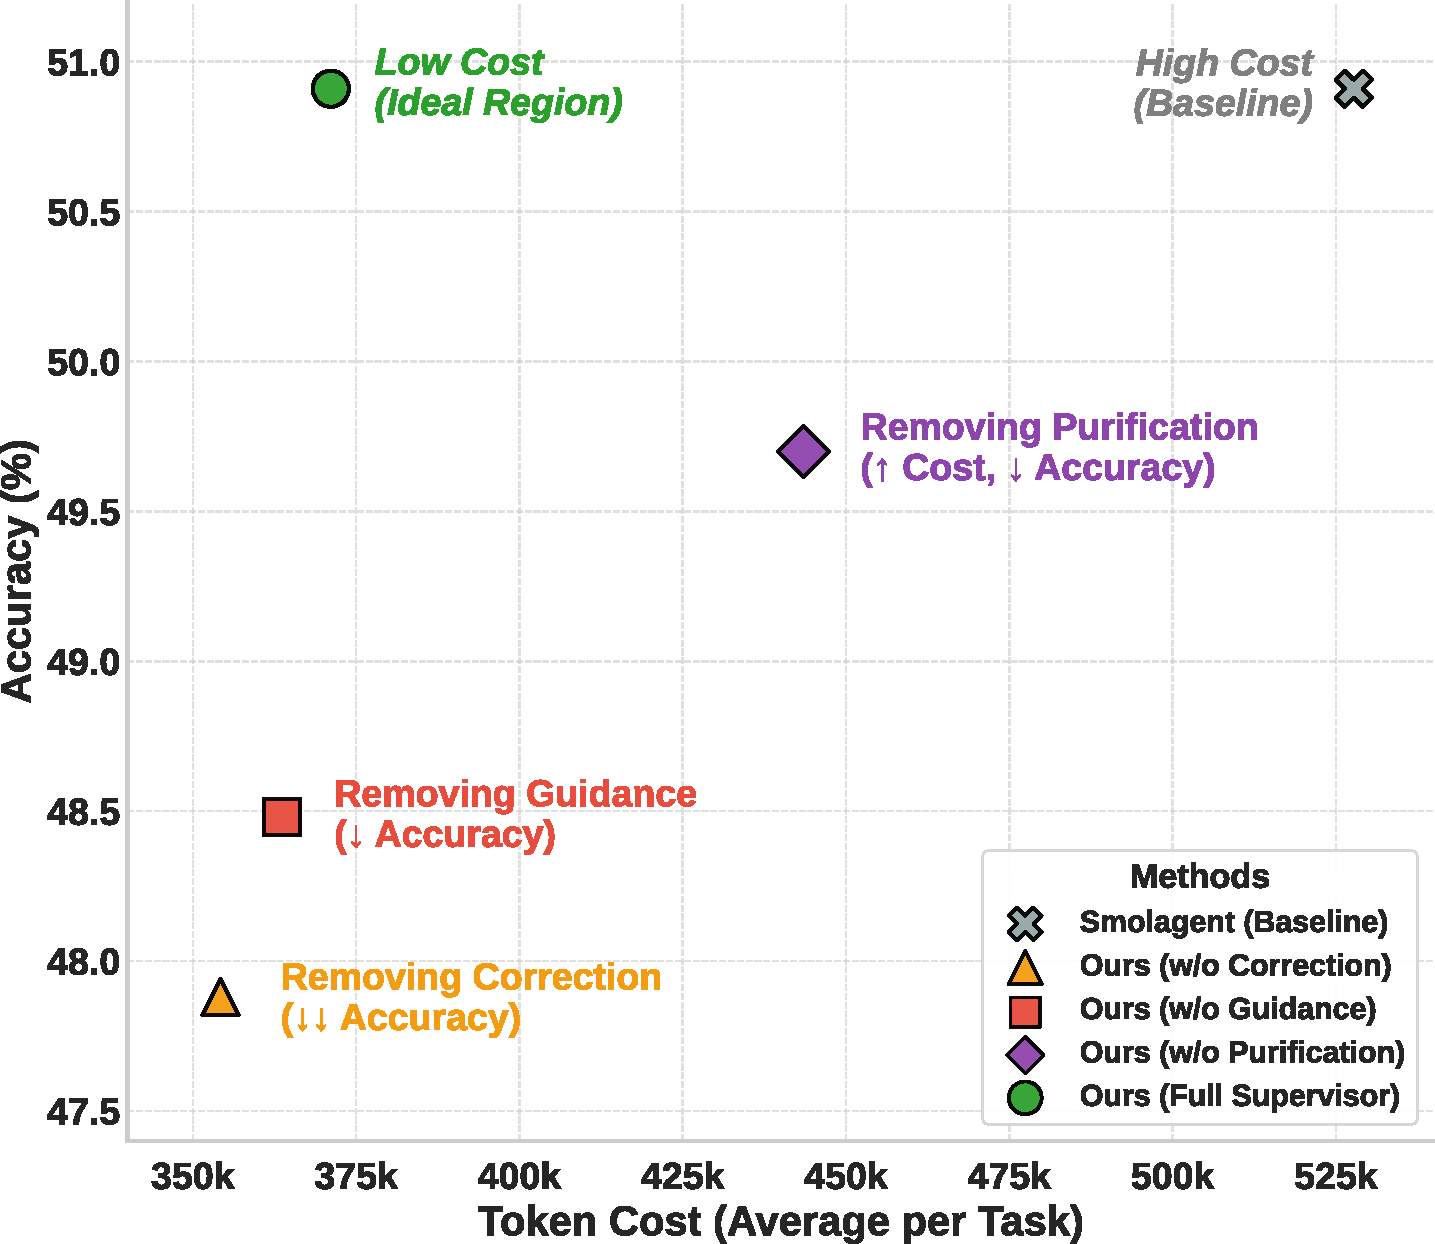
\includegraphics[width=\linewidth]{resources/figures/ablation_full.pdf}
        \caption{Ablation study on GAIA.}
        \label{fig:ablation}
    \end{subfigure}
    \hfill
    \begin{subfigure}[t]{0.45\textwidth}
        \centering
        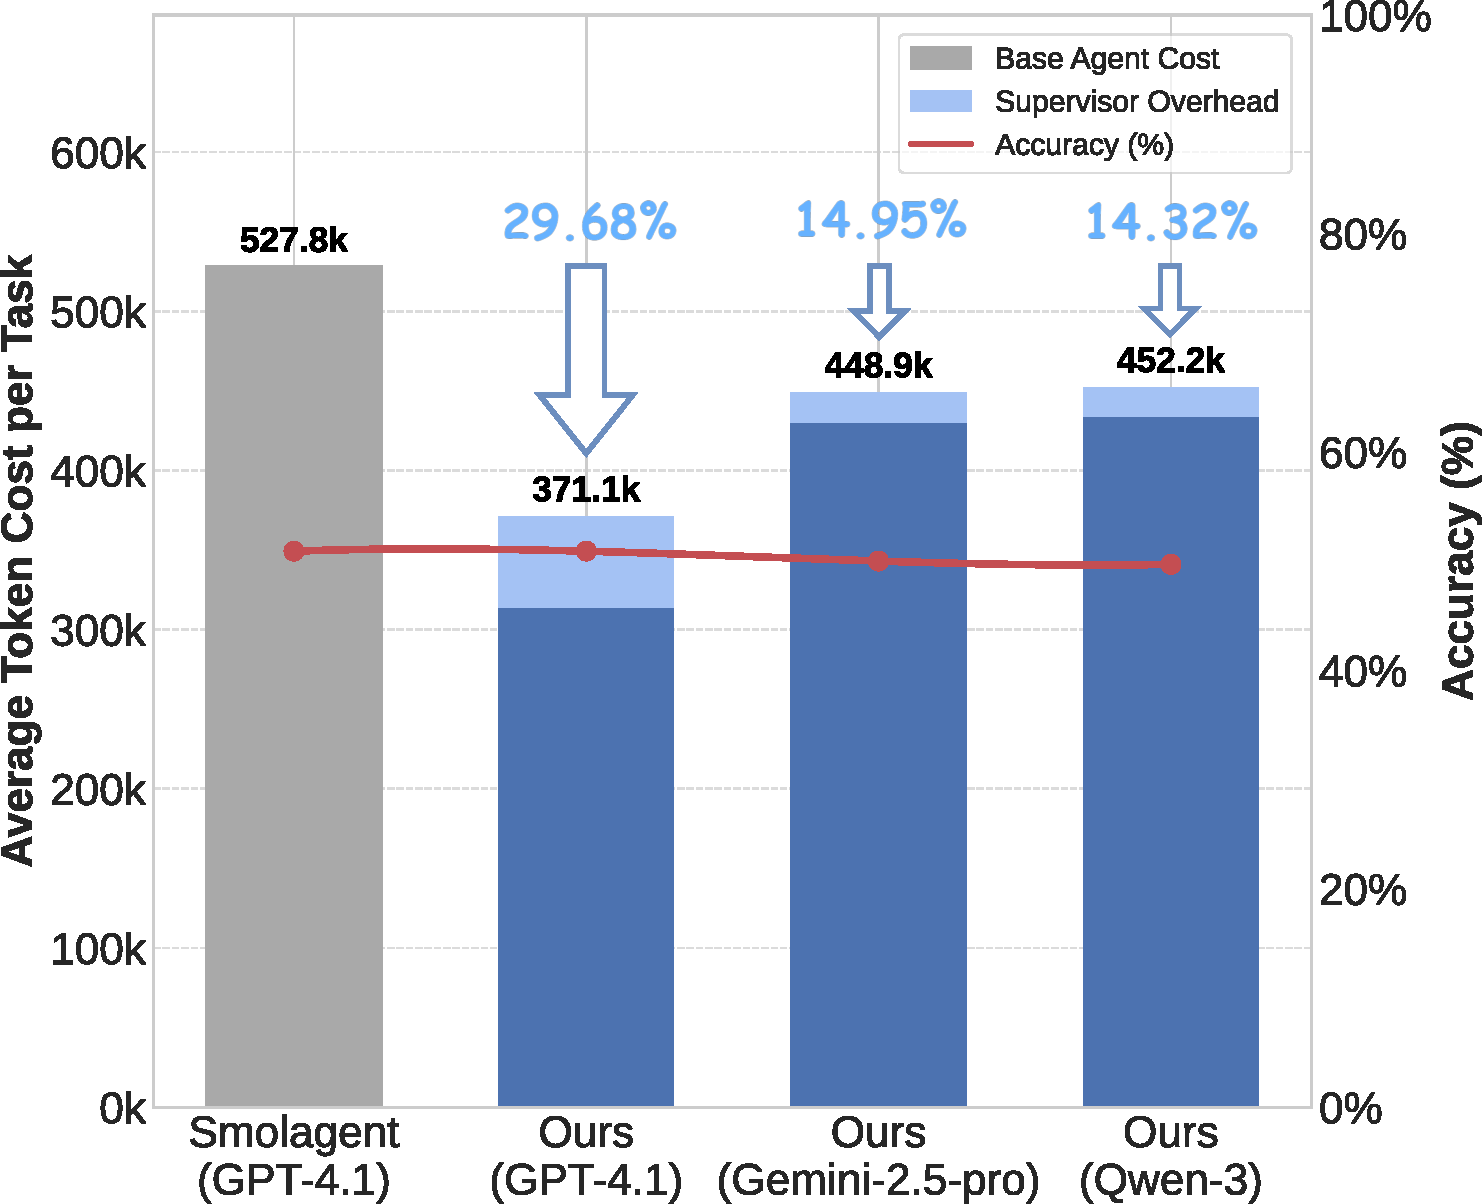
\includegraphics[width=\linewidth]{resources/figures/model_agnostic.pdf}
        \caption{Model Generalization of \method.}
        \label{fig:model-agnostic}
    \end{subfigure}
    \caption{
        \textbf{Ablation study and model generalization of \method.}
        \textbf{(a)}~Ablation study on challenging GAIA tasks, dissecting the distinct contributions of each module to the framework's overall efficiency and robustness.
        \textbf{(b)}~Validation of model-agnosticism, showing that \method consistently delivers token savings across diverse foundation models.
    }
    \label{fig:two-figs}
\end{figure}


\paragraph{MAS-Agnostic generalization.}
To verify MAS-agnostic feature of \method, we integrate \method into two distinct multi-agent system frameworks: AWorld~\citep{xie2025profileawaremaneuveringdynamicmultiagent} and OAgents~\citep{zhu2025oagentsempiricalstudybuilding}, and evaluate their performance on the subset of GAIA benchmark(top-10 most token-intensive tasks per GAIA level).
The results, presented in Table~\ref{tab:mas-agnostic}, indicate that \method consistently enhances the performance of both frameworks, underscoring its versatility and effectiveness across different MAS architectures.

Specifically, integrated with AWorld~\citep{xie2025profileawaremaneuveringdynamicmultiagent}, our SMAS(AWorld) achieved superior average accuracy over both the original AWorld (without Guard) and the Guard-enabled version. Furthermore, SMAS(AWorld) demonstrated substantial token efficiency, saving \textbf{36.54\%} on average versus AWorld (with Guard). With savings reaching \textbf{48.38\%} on Level 3 tasks, it confirms SMAS's ability to enhance tool-intensive MAS.
Applying \method to OAgents~\citep{zhu2025oagentsempiricalstudybuilding} further validated its general applicability, reducing average token consumption by \textbf{39.36\%} while maintaining competitive accuracy. Interestingly, the largest token reduction (\textbf{50.19\%}) occurred on Level 1 tasks, exceeding the savings on Level 3 (\textbf{40.63\%}). While this might reflect OAgents' inherent proficiency on harder tasks, the significant overall savings underscore \method's broad utility.

\paragraph{Overhead analysis.}
Crucially, all efficiency gains reported in this work represent \textbf{net savings}, fully accounting for the cost of \method. As detailed in Table \ref{tab:super_overhead}, the supervisor itself incurs a modest overhead, averaging only \textbf{15.45\%} of total token usage, which validates its lightweight design. Regarding latency, the supervisory interventions introduce an average increase of less than one minute and a half per task (Table \ref{tab:ablation_latency}). We consider this temporal cost a justifiable trade-off given the substantial economic savings achieved in complex multi-agent workflows. A comprehensive overhead analysis is provided in Appendix \ref{overhead_analysis}.

\begin{table}[!t]
    \caption{
        \textbf{Cross-framework performance of \method.}
        Evaluated on GAIA subset (top-10 most token-intensive tasks per level).
    }
    \label{tab:mas-agnostic}
    \centering
    \resizebox{\textwidth}{!}{
        \begin{tabular}{>{\raggedright\arraybackslash}m{4cm} c c c c c}
            \toprule
            \bf Method                  & \bf Avg. Acc.                                & \bf Avg. Token                                   & \bf Level 1 Avg. Token                           & \bf Level 2 Avg. Token                           & \bf Level 3 Avg. Token                           \\
            \midrule
            Smolagent                   & 40.00                                        & 1,446,526                                        & 933,013                                          & 2,037,437                                        & 1,369,131                                        \\
            \textbf{\, + SMAS}          & 46.67 {\scriptsize \textcolor{red}{↑6.67\%}} & 721,332 {\scriptsize \textcolor{blue}{↓50.13\%}} & 522,364 {\scriptsize \textcolor{blue}{↓44.01\%}} & 960,694 {\scriptsize \textcolor{blue}{↓52.85\%}} & 680,939 {\scriptsize \textcolor{blue}{↓50.26\%}} \\ \midrule
            AWorld (without Guard)      & 23.33                                        & 155,239                                          & 50,851                                           & 217,332                                          & 166,500                                          \\
            AWorld (with Guard)         & 30.00                                        & 353,738                                          & 135,413                                          & 463,083                                          & 376,878                                          \\
            \textbf{AWorld (with SMAS)} & 36.67 {\scriptsize \textcolor{red}{↑6.67\%}} & 224,480 {\scriptsize \textcolor{blue}{↓36.54\%}} & 90,569 {\scriptsize \textcolor{blue}{↓33.12\%}}  & 355,051 {\scriptsize \textcolor{blue}{↓23.33\%}} & 194,561 {\scriptsize \textcolor{blue}{↓48.38\%}} \\ \midrule
            OAgents                     & 46.67                                        & 530,939                                          & 430,852                                          & 359,511                                          & 802,454                                          \\
            \textbf{\, + SMAS}          & 46.67                                        & 321,957 {\scriptsize \textcolor{blue}{↓39.36\%}} & 214,604 {\scriptsize \textcolor{blue}{↓50.19\%}} & 274,875 {\scriptsize \textcolor{blue}{↓23.54\%}} & 476,393 {\scriptsize \textcolor{blue}{↓40.63\%}} \\
            \bottomrule
        \end{tabular}
    }
\end{table}


\section{Discussion and Conclusion}

\paragraph{Supervisor as a foundational MAS component.}

Our work positions \method as a foundational component for future Multi-Agent Systems, akin to established modules like memory banks and tool-usage frameworks. By providing real-time, adaptive supervision, \method alleviates critical challenges of robustness and efficiency that are pervasive across diverse MAS architectures. Its modular design allows for seamless integration with existing systems, enhancing their performance without necessitating fundamental changes to their core logic. This underscores the potential of supervisory agents as universal enhancers of MASs, capable of elevating both reliability and cost-effectiveness across a wide range of applications.

\paragraph{Comparison with related supervisory agents.}
A related concept is the Guard agent in AWorld~\citep{xie2025profileawaremaneuveringdynamicmultiagent}, which is invoked at key steps primarily for factual verification to enhance task accuracy. While valuable, its scope differs significantly from our method. \method{} adopts a broader objective of improving overall system efficiency and robustness through continuous (albeit adaptively filtered) monitoring and a wider range of interventions, including error correction, inefficiency guidance, and observation purification, complementing the Guard's focus on accuracy.

\paragraph{Broader insights.}

Our work also yields critical insights for the broader field. First, we discovered that seemingly “noisy” information, such as HTML structure and truncation cues, serves as a vital signal for ReAct-style agents. The overly aggressive purification can paradoxically harm performance. This highlights a fundamental trade-off between information density and the preservation of environmental texture.
Second, our focus on token cost underscores the need for a more holistic efficiency evaluation for MAS. A comprehensive analysis must also account for the frequency and complexity of external tool API calls, which offload significant burdens from the MAS.
This very trade-off informed our choice of Smolagent as a primary testbed - its reliance on internal agentic reasoning, rather than powerful external tools, provided a controlled environment to isolate and evaluate our \method's impact on the interaction process itself.

\paragraph{Future directions.}
These insights inform several promising avenues for future work. First, moving beyond heuristic rules, exploring a learning-based adaptive filter could enable more precise, dynamic control over supervisor invocations. This aligns with the broader goal of developing a self-evolving, memory-augmented version of \method{}. Second, further research should focus on mitigating the latency overhead introduced by supervisory calls to enhance real-time applicability, alongside creating sophisticated purification techniques that address the ``noise-as-signal'' trade-off. Finally, developing a universal resource consumption metric for MAS remains a critical open challenge. Ultimately, we posit that incorporating such real-time, meta-level supervision is a foundational component for building the next generation of truly scalable and reliable MAS.

\paragraph{Conclusion.}

In this work, we introduced \textbf{\method}, a lightweight and non-intrusive meta-agent framework that enhances the robustness and efficiency of Multi-Agent Systems. Through real-time, adaptive supervision, \method{} mitigates common failure modes and reduces computational overhead using three core strategies: proactive error correction, pragmatic inefficiency guidance, and adaptive observation purification. Our extensive experiments demonstrate a significant Pareto improvement. On the challenging GAIA benchmark, \method{} reduces token consumption by an average of 29.68\% while maintaining competitive task success rates, a crucial step towards building more practical and scalable agentic systems.
